\chapter{Исследовательская часть}

В данном разделе будут приведены технические характеристики устройства, на котором проводился анализ алгоритмов, а также результаты работы программного обеспечения.

\section{Технические характеристики}

Технические характеристики устройства, на котором выполнялось исследование, следующие:

\begin{itemize}[label=---]
	\item Операционная система: Microsoft Windows 10 Pro;
	\item Оперативная память: 32 ГБ;
	\item Процессор: Intel(R) Core(TM) i9-9980HK CPU @ 2.40GHz, 2401 Mhz;
	\item Количество ядер: 8 физических и 16 логических.
\end{itemize}

\section{Результаты работы ПО}

На рисунках \ref{img:4-1} -- \ref{img:4-5} представлены изображения, полученные с помощью разработанного ПО.

\begin{table}[H]
	\centering
	\begin{tabular}{p{1\linewidth}}
		\centering
		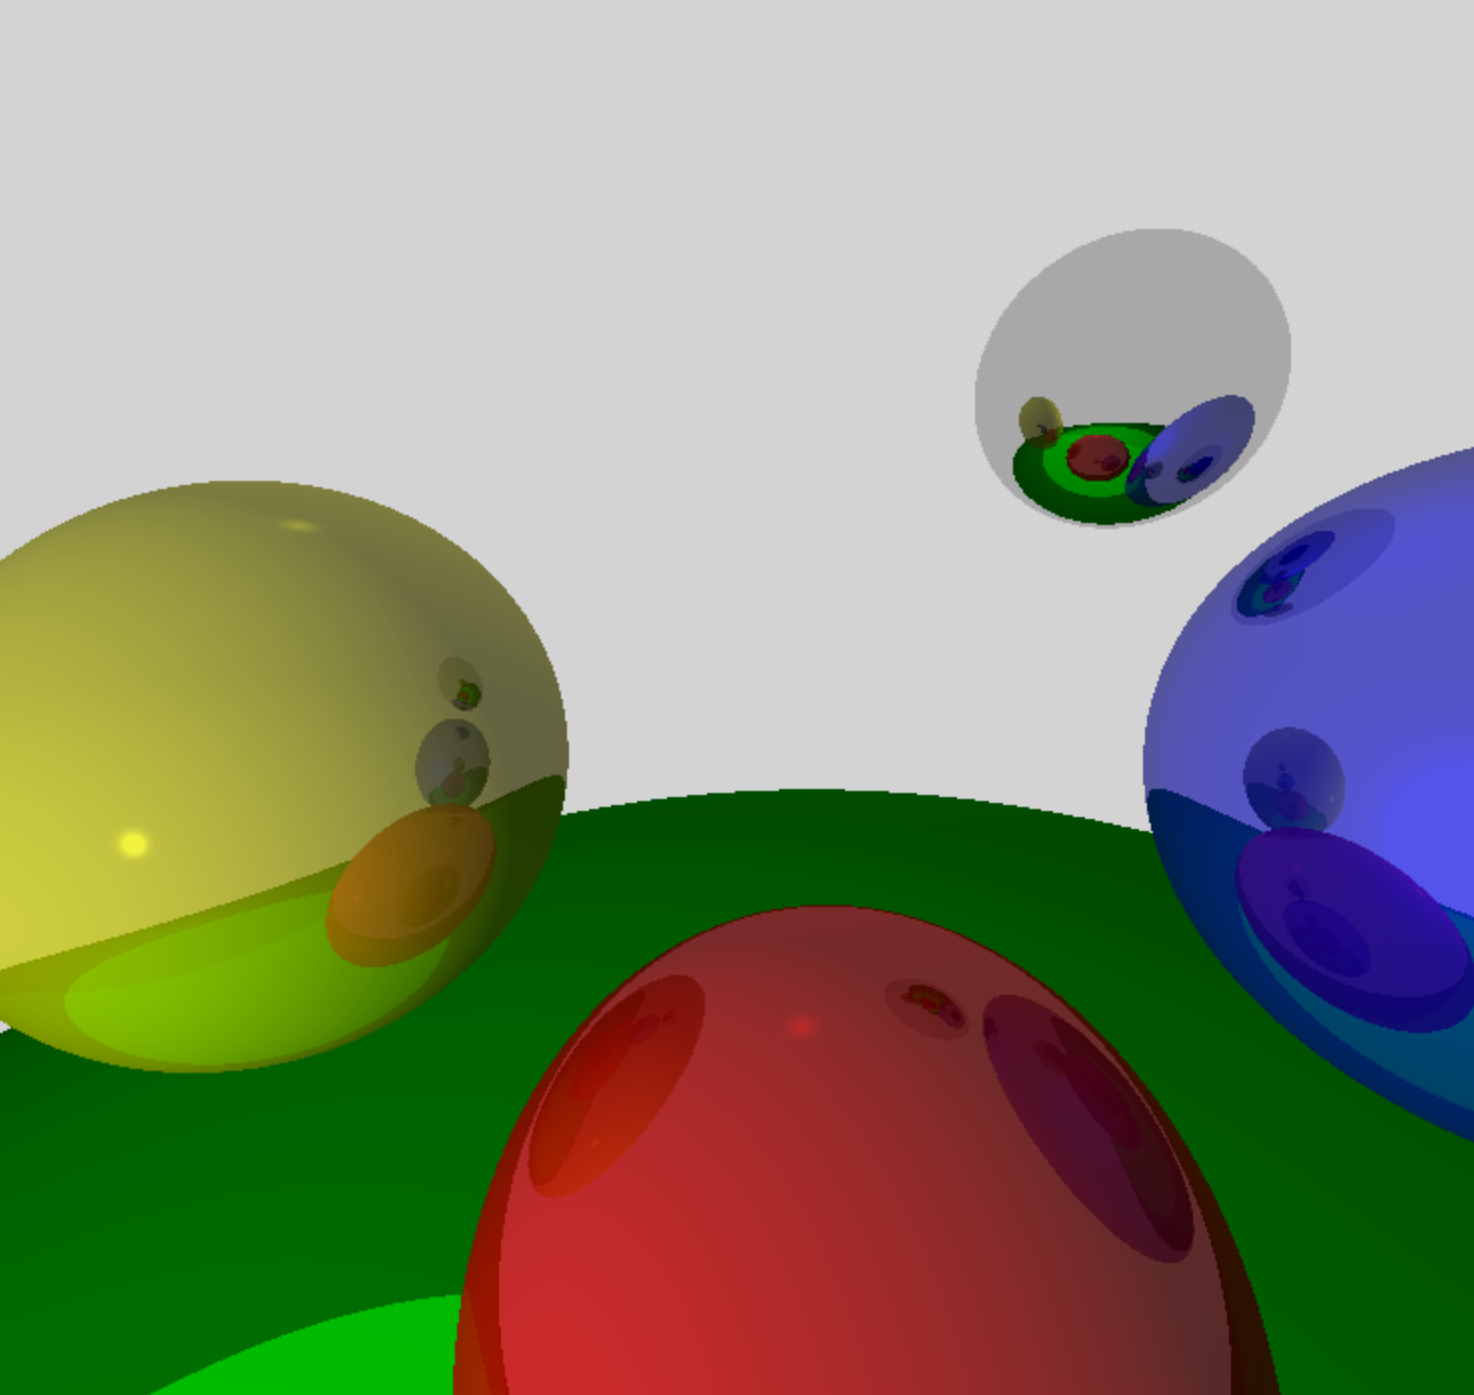
\includegraphics[width=0.55\linewidth]{include/4-1.png}
		\captionof{figure}{Отражение сфер друг от друга.}
		\label{img:4-1}
	\end{tabular}
\end{table}

\begin{table}[H]
	\centering
	\begin{tabular}{p{1\linewidth}}
		\centering
		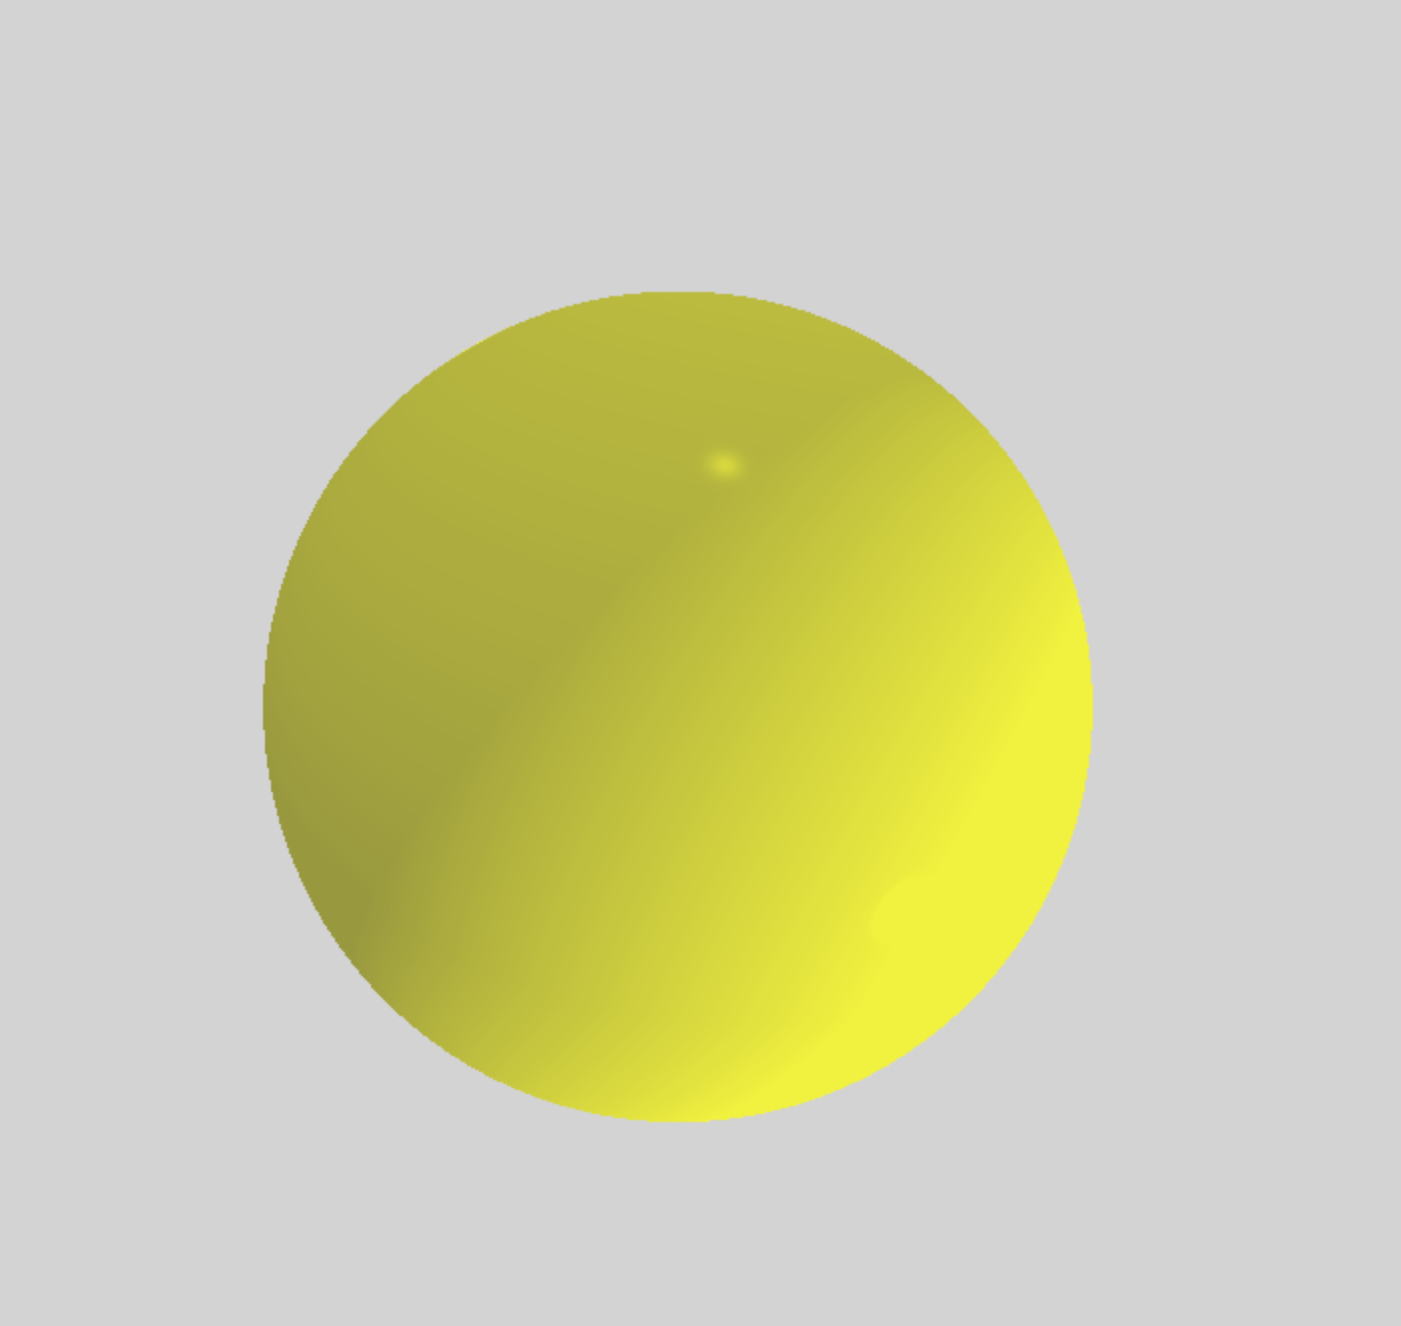
\includegraphics[width=0.55\linewidth]{include/4-2.png}
		\captionof{figure}{Отображение света.}
		\label{img:4-2}
	\end{tabular}
\end{table}

\begin{table}[H]
	\centering
	\begin{tabular}{p{1\linewidth}}
		\centering
		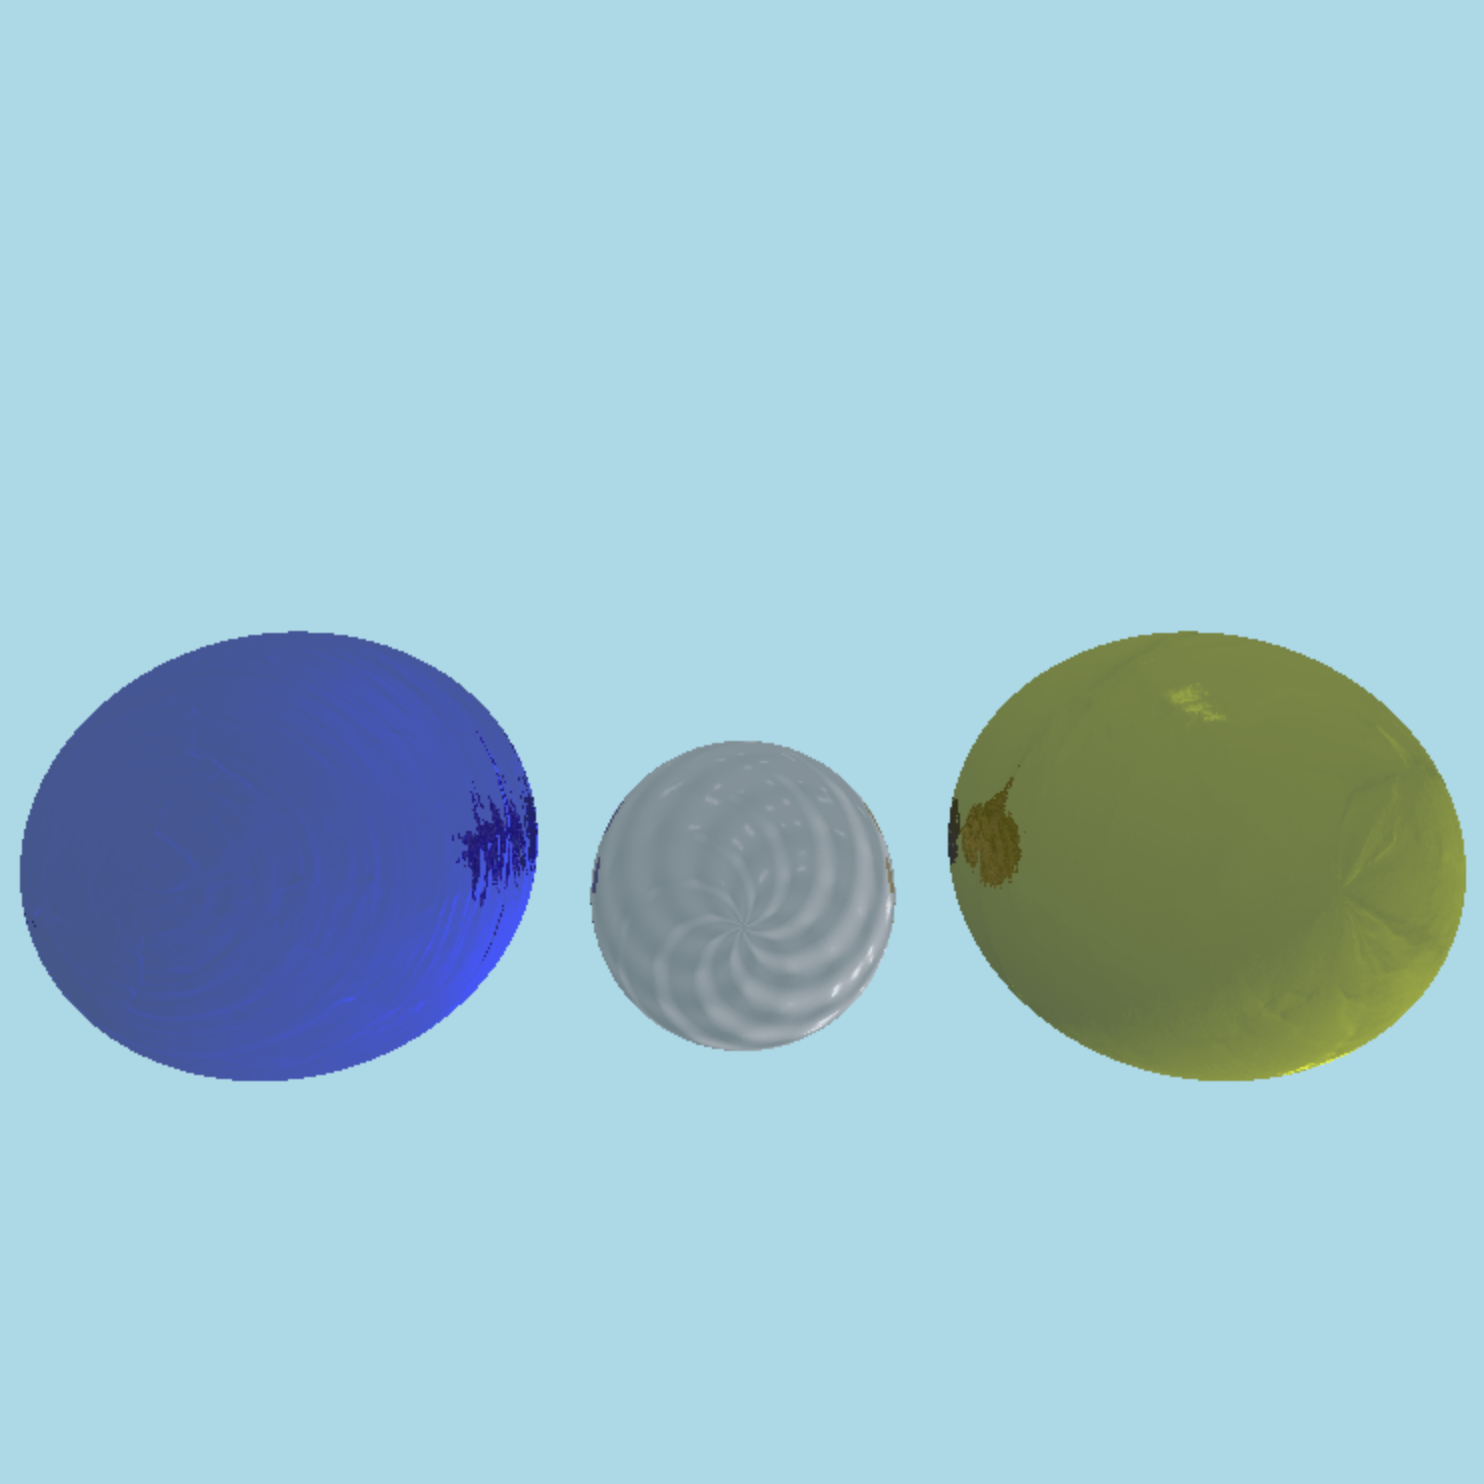
\includegraphics[width=0.55\linewidth]{include/4-4.png}
		\captionof{figure}{Простая композиция шаров с текстурами, наложенными по карте высот.}
		\label{img:4-3}
	\end{tabular}
\end{table}

\begin{table}[H]
	\centering
	\begin{tabular}{p{1\linewidth}}
		\centering
		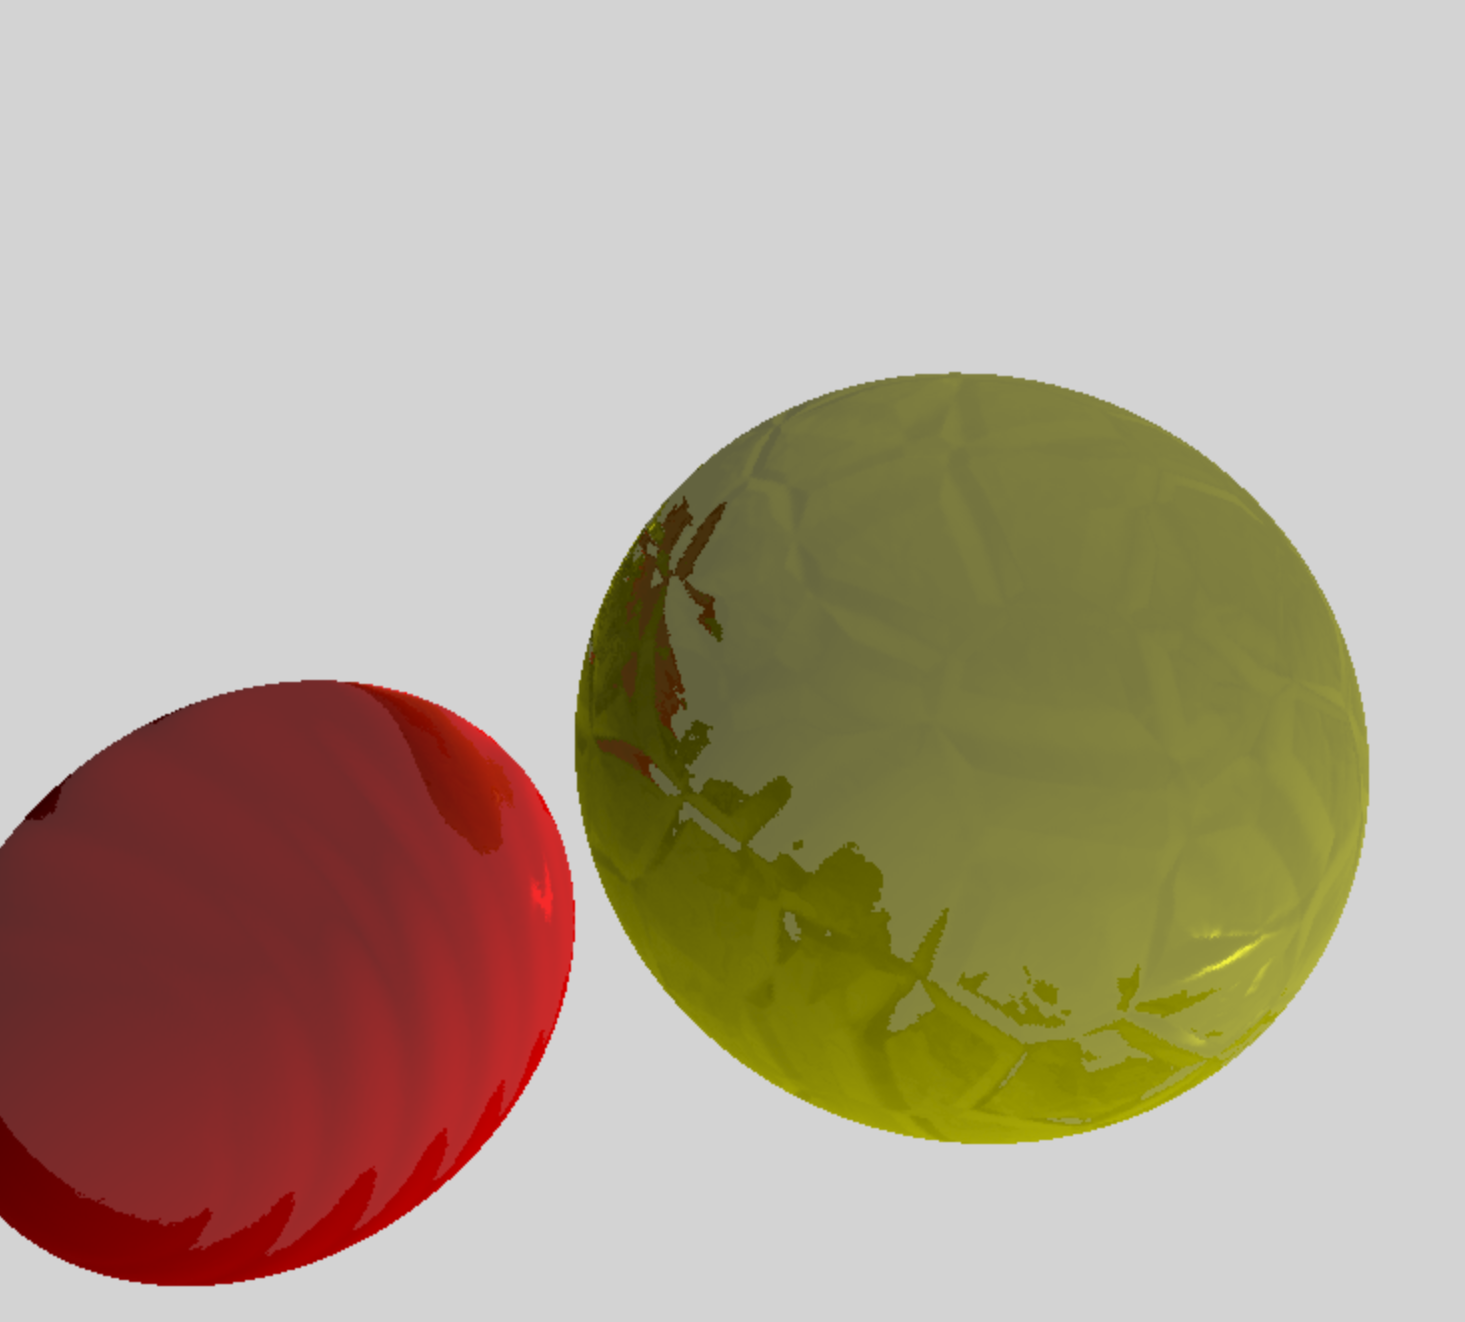
\includegraphics[width=0.55\linewidth]{include/4-3.png}
		\captionof{figure}{Простая композиция шаров с текстурами, наложенными по карте нормалей.}
		\label{img:4-4}
	\end{tabular}
\end{table}

\begin{table}[H]
	\centering
	\begin{tabular}{p{1\linewidth}}
		\centering
		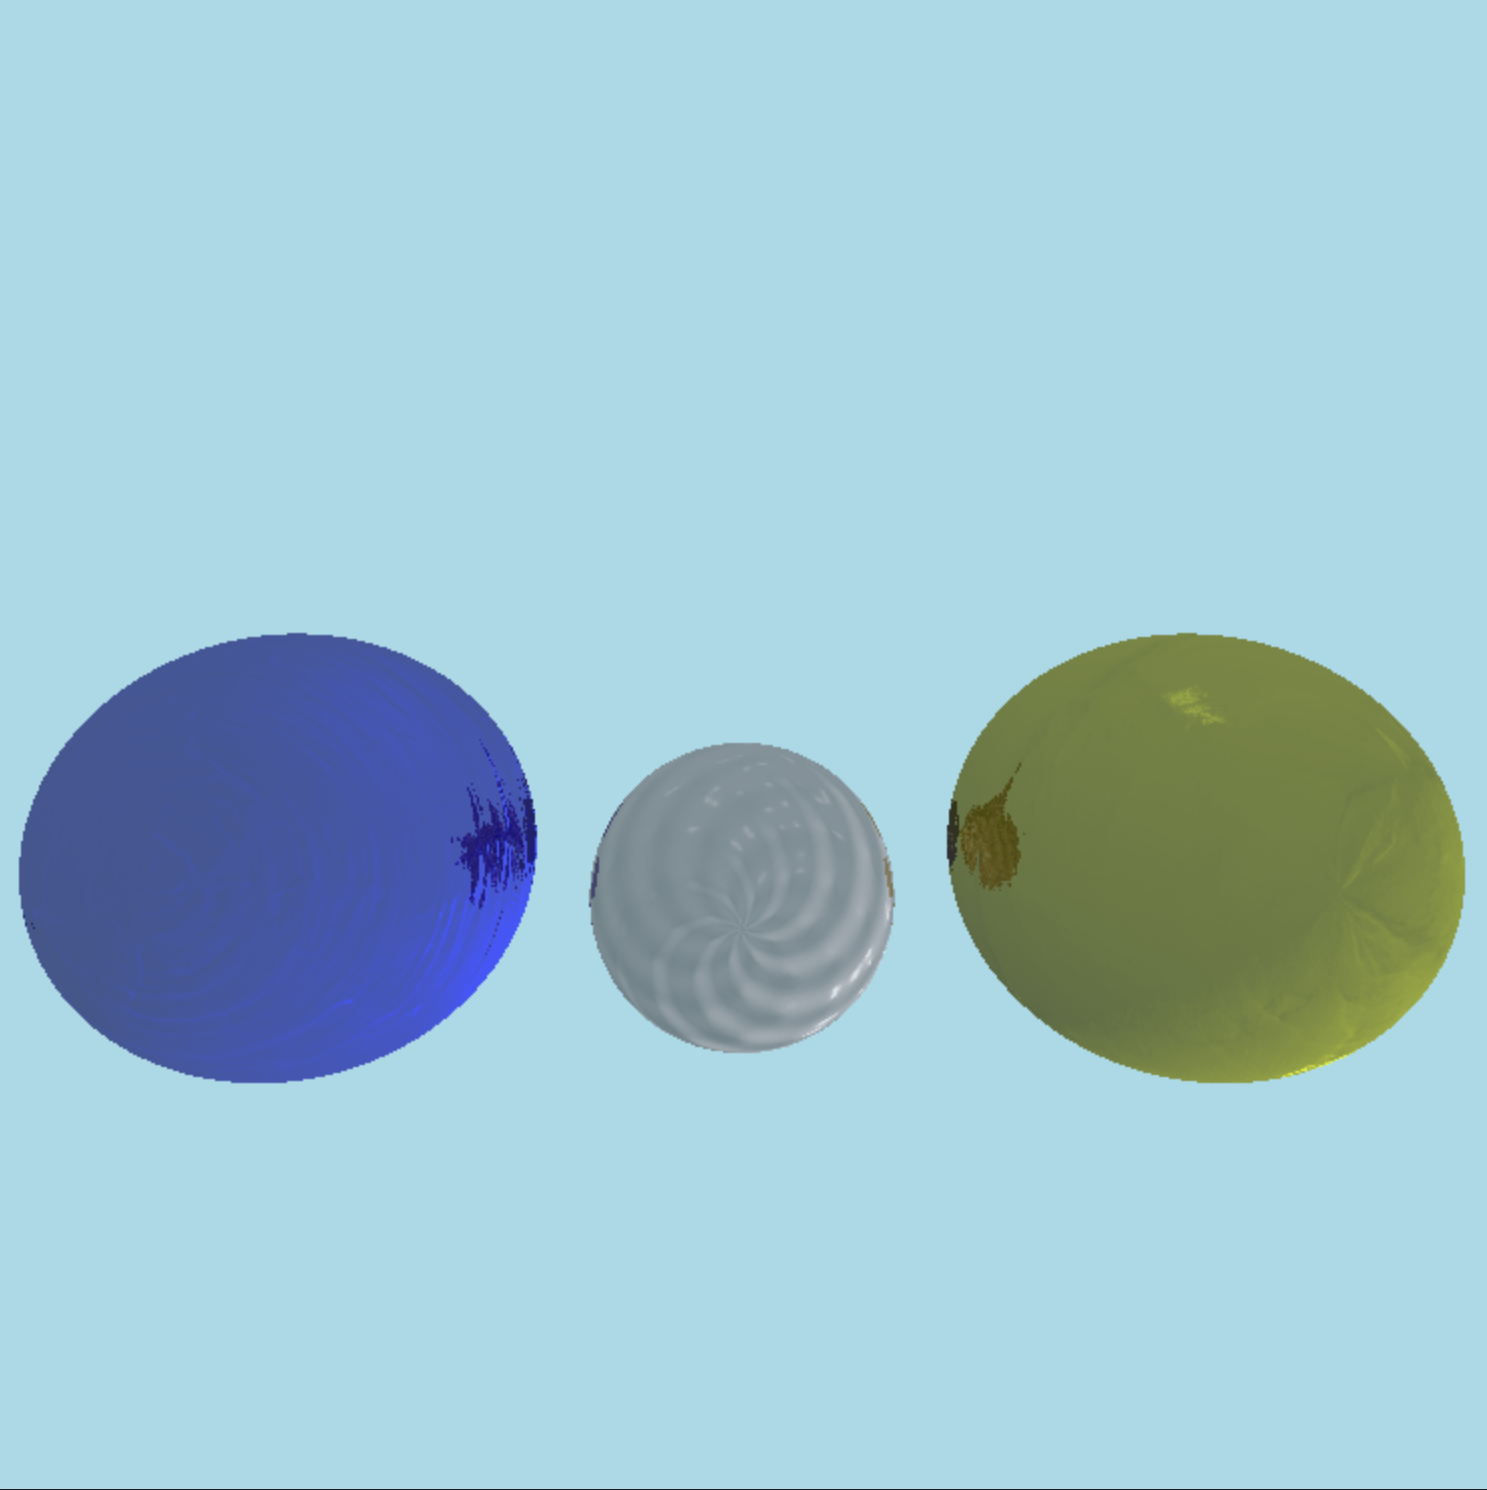
\includegraphics[width=0.55\linewidth]{include/4-5.png}
		\captionof{figure}{Простая композиция шаров с текстурами, наложенными по карте паралактического отображения.}
		\label{img:4-5}
	\end{tabular}
\end{table}

\section{Анализ наложения текстур}

Как мы можем заметить, на получившихся сценах (\ref{img:4-1} -- \ref{img:4-5}) текстуры накладываются визуально схожим образом, все три варианта содержать правильное отображение теней, бликов и отражений. Таким образом на практике применимы все варианты, но чтобы более точно проанализировать эти методы, проведем еще одну проверку.

Согласно теории, методы наложения текстур по карте высот и нормалей очень схожи, просто по-разному хранятся данные. А для текстурирования по картам параллактического отображения, нам нужны дополнительные математические вычисления, но в итоге должна выйти более привлекательная сцена в тех местах, где мы смотрим на объект под маленьким углом. Чтобы в этом убедиться построим сцену, где мы будем нахожится ближе к поверхности большого шара и будем смотреть вдоль нее. Результаты работы программы с такой сценой представлены на рисунках \ref{img:4-6} -- \ref{img:4-8}.

\begin{table}[H]
	\centering
	\begin{tabular}{p{1\linewidth}}
		\centering
		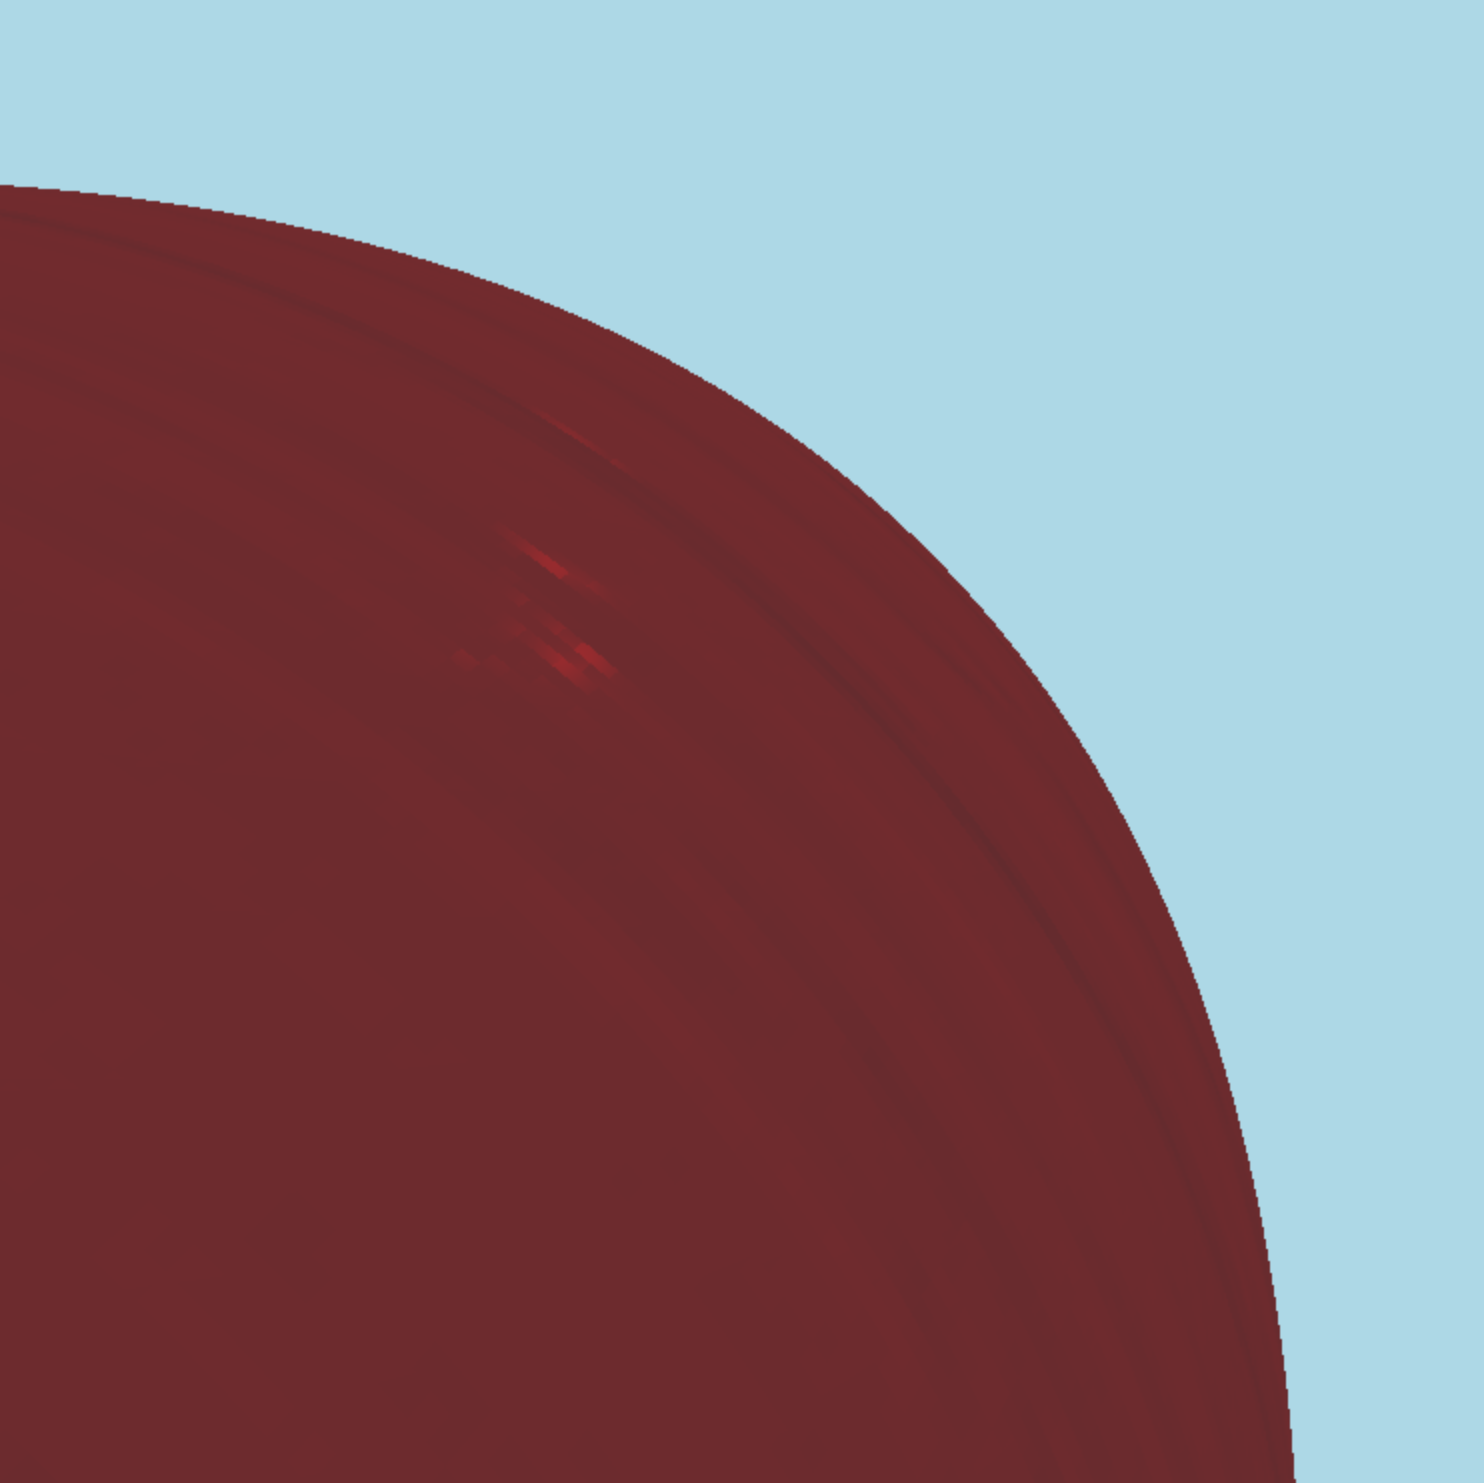
\includegraphics[width=0.55\linewidth]{include/4-6.png}
		\captionof{figure}{Поверхность шара под маленьким углом с текстурами, наложенными по карте высот.}
		\label{img:4-6}
	\end{tabular}
\end{table}

\begin{table}[H]
	\centering
	\begin{tabular}{p{1\linewidth}}
		\centering
		
\includegraphics[width=0.55\linewidth]{include/4-7.png}
		\captionof{figure}{Поверхность шара под маленьким углом с текстурами, наложенными по карте нормалей.}
		\label{img:4-7}
	\end{tabular}
\end{table}

\begin{table}[H]
	\centering
	\begin{tabular}{p{1\linewidth}}
		\centering
		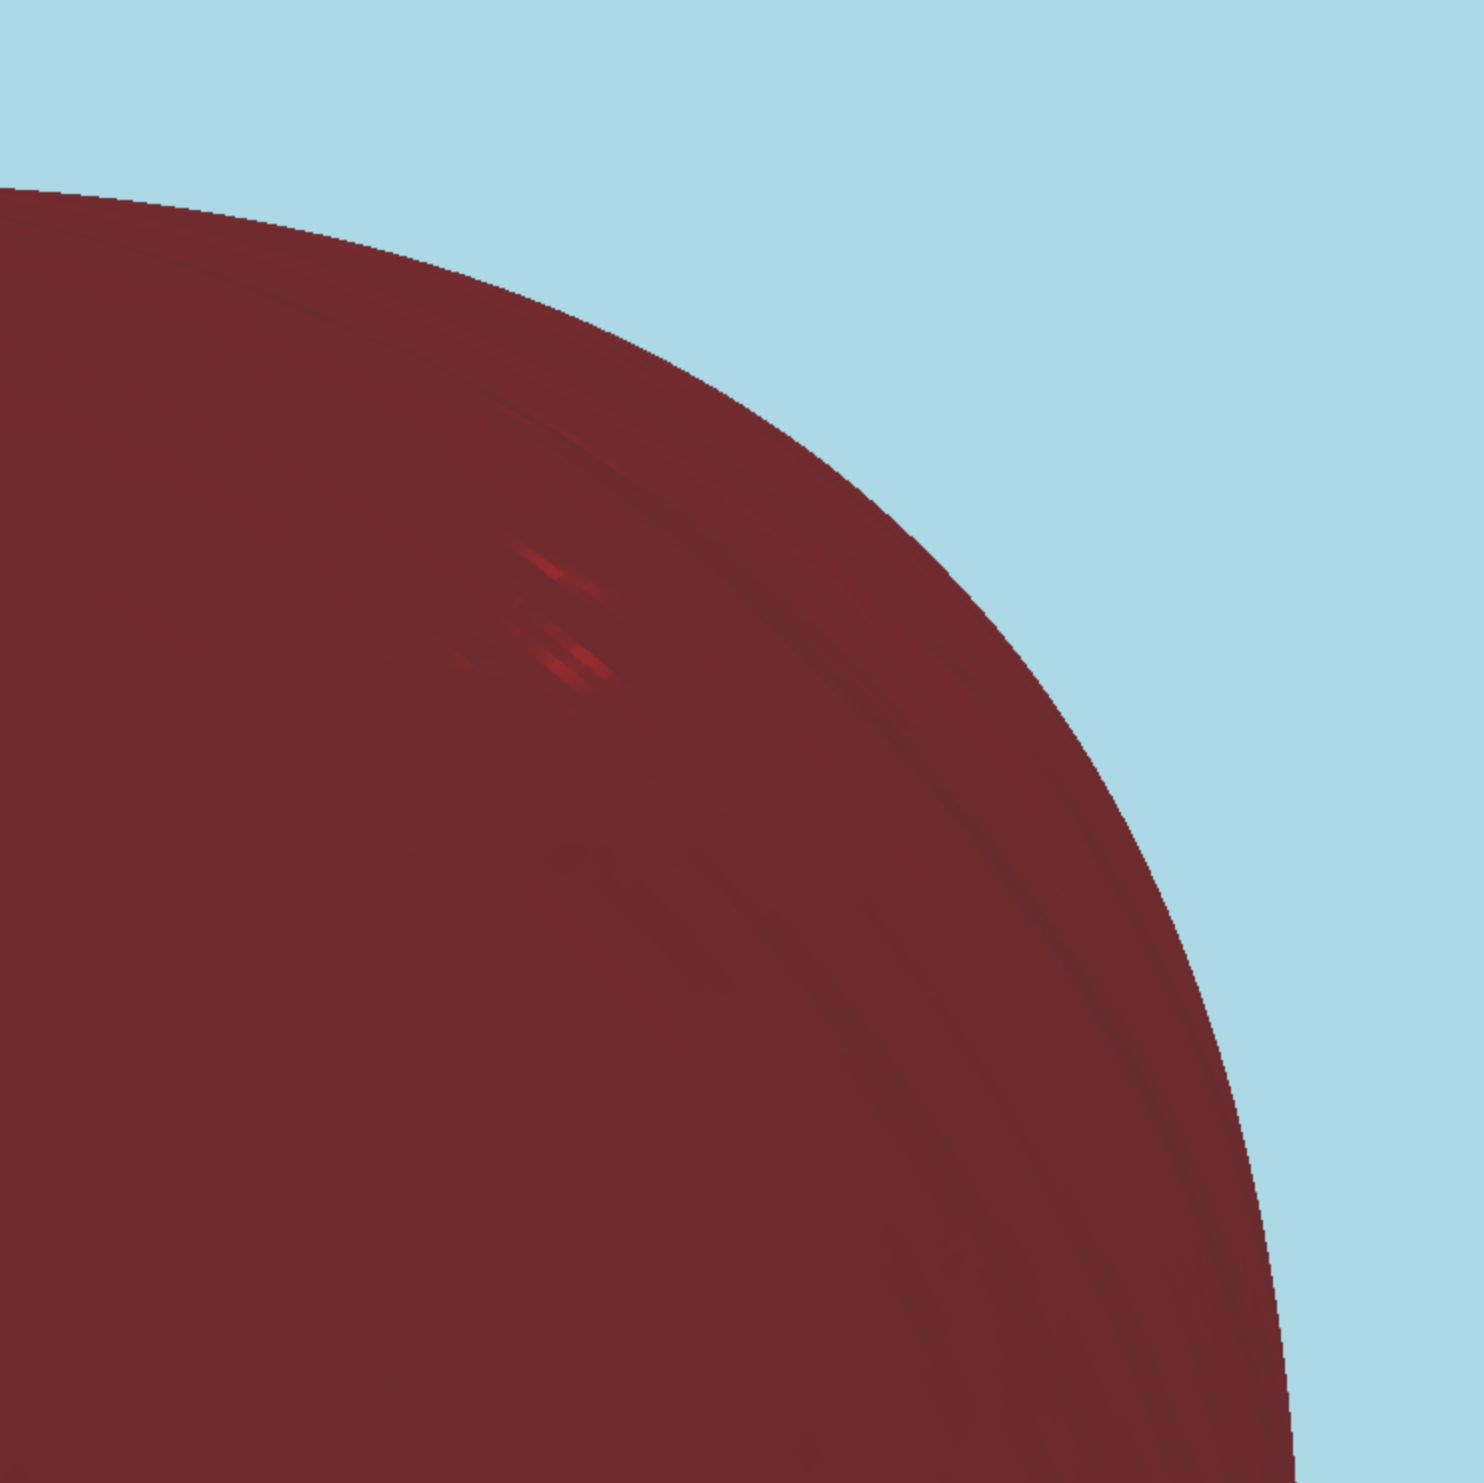
\includegraphics[width=0.55\linewidth]{include/4-8.png}
		\captionof{figure}{Поверхность шара под маленьким углом с текстурами, наложенными по карте паралактического отображения.}
		\label{img:4-8}
	\end{tabular}
\end{table}

Сравнивая полученные изображения можно с уверенностью сказать что улучшения, которые дает нам параллакс действительно видны, и в работах, требующих визуализации, более приближенной к реальности, такой алгоритм вполне подойдет. Что касается карты нормалей -- поскольку там нет математических вычислений и возмущение полностью заложено в текстурную карту, результат получается более точным. Такой вариант подойдет, когда мы можем отдавать приоритет анализу больших данных, нежели вычислениям.

\section{Анализ производительности}

Для завершения исследования осталось проверить скорость выполнения алгоритом. Для этого рассмотрим сцены разной степени нагруженности по количеству шаров, а так же разные способы наложения текстур.
Результаты работы программы приведены в таблице \ref{tbl:tab-1}. 

\begin{table}[H]
	\begin{center}
		\caption{\label{tbl:tab-1} Производительность ПО при разном размере тканевой сетки.}
		\begin{tabular}{|c|c|c|c|}
			\hline
			\specialcell{Номер} & \specialcell{Карта высот.} & \specialcell{Карта нормалей.} & \specialcell{Карта параллакса.}
			\\
			\specialcell{сцены} & \specialcell{Время работы, мс.} & \specialcell{Время работы, мс.} & \specialcell{Время работы, мс.}
			\\ \hline
			1 & 301.1235 & 524.8413 & 429.1257 \\ \hline
			2 & 446.9992 & 671.1294 & 558.0016 \\ \hline
			3 & 512.6823 & 790.8529 & 602.9895 \\ \hline
			4 & 632.1282 & 993.8422 & 767.7887 \\ \hline
			5 & 728.1388 & 1053.046 & 950.8592 \\ \hline
			6 & 1068.7003 & 1514.2481 & 1168.2758 \\ \hline
			7 & 1388.5561 & 3143.9859 & 1401.0582 \\ \hline
		\end{tabular}
	\end{center}
\end{table}

По результатам исследования времени работы ПО мы видим, что самым эффективным способом текстурирования является наложение карт высот, чуть медленнее -- карт параллакса, и самым неудачным способом -- использование карт нормалей.

\section*{Вывод}
В данном разделе были представлены результаты работы ПО, проанализировано наложение текстур, а так же время работы программы. В итоге было выявлено, что самым менее затратным по времени, и при этом достаточно наглядным, является наложение текстур с помощью карт высот. Более визуально точным является наложение текстур по параллаксу, но это требует чуть больше времени. Самым визуально точным является текстурирование по картам нормалей, что требует самого большого количества времени, которое сильно растет с усложнением сцены. Это может вызвать больше проблемы с производительностью, поэтому такой метод стоит внедрять только с более проработанной обработкой больших данных.